% Figure 1: Authoring ablation gradient (A0-A6) vs Reviewer ablation gradient (C0-C6)
% Self-contained figure environment — \input{} into main.tex.
% Requires: pgfplots, subcaption (loaded in main preamble).

\begin{figure*}[t]
  \centering

  % ---------------------------------------------------------------
  % LEFT: Authoring ablation A0-A6 (/45, pass threshold = 33)
  % ---------------------------------------------------------------
  \begin{subfigure}[t]{0.47\textwidth}
    \centering
    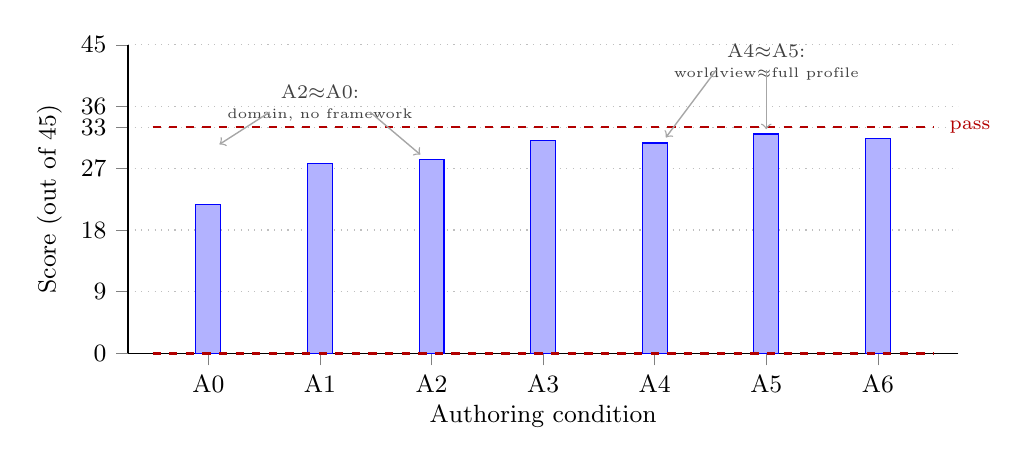
\begin{tikzpicture}
      \begin{axis}[
          ybar,
          bar width        = 9pt,
          width            = \textwidth,
          height           = 5.5cm,
          ymin             = 0,
          ymax             = 45,
          ytick            = {0,9,18,27,33,36,45},
          yticklabels      = {0,9,18,27,33,36,45},
          xtick            = data,
          xticklabels      = {A0,A1,A2,A3,A4,A5,A6},
          xticklabel style = {font=\small},
          yticklabel style = {font=\small},
          ylabel           = {Score (out of 45)},
          ylabel style     = {font=\small},
          xlabel           = {Authoring condition},
          xlabel style     = {font=\small, yshift=2pt},
          enlarge x limits = 0.12,
          axis x line*     = bottom,
          axis y line*     = left,
          tick align       = outside,
          ymajorgrids      = true,
          grid style       = {dotted, gray!50},
          every axis plot/.append style = {fill=blue!55, draw=blue!70!black},
          clip             = false,
        ]

        % Bar data
        \addplot coordinates {
          (0, 21.7)
          (1, 27.7)
          (2, 28.3)
          (3, 31.0)
          (4, 30.7)
          (5, 32.0)
          (6, 31.3)
        };

        % Pass-threshold dashed line at y=33
        \draw[dashed, red!70!black, line width=0.8pt]
          ({rel axis cs:0,0} -| {axis cs:-0.5,0}) --
          ({rel axis cs:1,0} -| {axis cs: 6.5,0})
          node[right, font=\scriptsize, text=red!70!black] {}; % drawn via extra draw below

        \draw[dashed, red!70!black, line width=0.8pt]
          (axis cs:-0.5, 33) -- (axis cs:6.5, 33)
          node[pos=1.0, right, font=\scriptsize, text=red!70!black, xshift=2pt]
          {pass};

        % Annotation: A0 ≈ A2 (domain without framework)
        % Arrow from label above bars 0 and 2
        \node[font=\scriptsize, align=center, text=black!75]
          at (axis cs:1, 36.5)
          {A2$\approx$A0:\\[-1pt]{\tiny domain, no framework}};
        \draw[->, gray!70, line width=0.5pt]
          (axis cs:0.55, 35.2) -- (axis cs:0.1, 30.5);
        \draw[->, gray!70, line width=0.5pt]
          (axis cs:1.45, 35.2) -- (axis cs:1.9, 29.0);

        % Annotation: A4 ≈ A5 (worldview ≈ full profile)
        \node[font=\scriptsize, align=center, text=black!75]
          at (axis cs:5, 42.5)
          {A4$\approx$A5:\\[-1pt]{\tiny worldview$\approx$full profile}};
        \draw[->, gray!70, line width=0.5pt]
          (axis cs:4.55, 41.3) -- (axis cs:4.1, 31.5);
        \draw[->, gray!70, line width=0.5pt]
          (axis cs:5.0, 41.3) -- (axis cs:5.0, 32.7);

      \end{axis}
    \end{tikzpicture}
    \caption{Authoring ablation (A0--A6).}
    \label{fig:gradients:authoring}
  \end{subfigure}
  %
  \hfill
  %
  % ---------------------------------------------------------------
  % RIGHT: Reviewer ablation C0-C6 (/30, pass threshold = 22)
  % ---------------------------------------------------------------
  \begin{subfigure}[t]{0.47\textwidth}
    \centering
    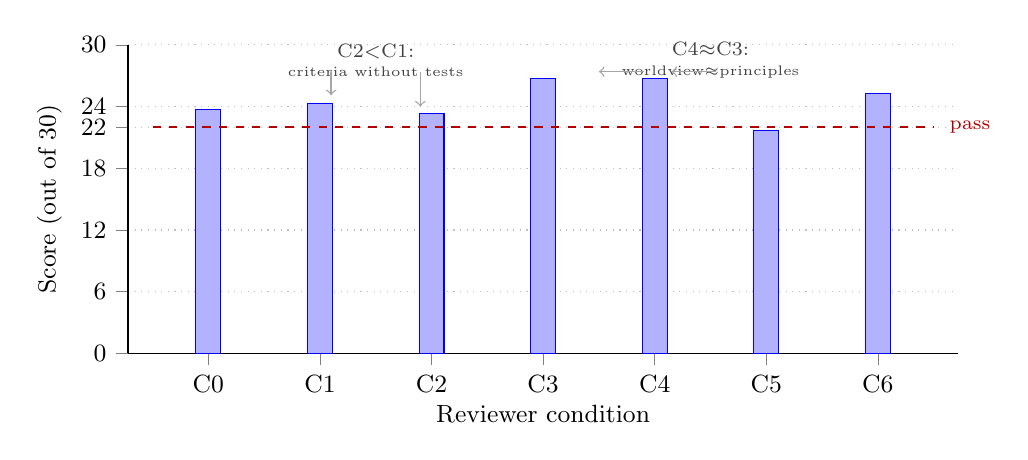
\begin{tikzpicture}
      \begin{axis}[
          ybar,
          bar width        = 9pt,
          width            = \textwidth,
          height           = 5.5cm,
          ymin             = 0,
          ymax             = 30,
          ytick            = {0,6,12,18,22,24,30},
          yticklabels      = {0,6,12,18,22,24,30},
          xtick            = data,
          xticklabels      = {C0,C1,C2,C3,C4,C5,C6},
          xticklabel style = {font=\small},
          yticklabel style = {font=\small},
          ylabel           = {Score (out of 30)},
          ylabel style     = {font=\small},
          xlabel           = {Reviewer condition},
          xlabel style     = {font=\small, yshift=2pt},
          enlarge x limits = 0.12,
          axis x line*     = bottom,
          axis y line*     = left,
          tick align       = outside,
          ymajorgrids      = true,
          grid style       = {dotted, gray!50},
          every axis plot/.append style = {fill=teal!60, draw=teal!80!black},
          clip             = false,
        ]

        % Bar data
        \addplot coordinates {
          (0, 23.7)
          (1, 24.3)
          (2, 23.3)
          (3, 26.7)
          (4, 26.7)
          (5, 21.7)
          (6, 25.3)
        };

        % Pass-threshold dashed line at y=22
        \draw[dashed, red!70!black, line width=0.8pt]
          (axis cs:-0.5, 22) -- (axis cs:6.5, 22)
          node[pos=1.0, right, font=\scriptsize, text=red!70!black, xshift=2pt]
          {pass};

        % Annotation: C2 < C1 (criteria without tests)
        \node[font=\scriptsize, align=center, text=black!75]
          at (axis cs:1.5, 28.5)
          {C2$<$C1:\\[-1pt]{\tiny criteria without tests}};
        \draw[->, gray!70, line width=0.5pt]
          (axis cs:1.1, 27.4) -- (axis cs:1.1, 25.1);
        \draw[->, gray!70, line width=0.5pt]
          (axis cs:1.9, 27.4) -- (axis cs:1.9, 24.0);

        % Annotation: C4 ≈ C3 (worldview ≈ principles)
        \node[font=\scriptsize, align=center, text=black!75]
          at (axis cs:4.5, 28.5)
          {C4$\approx$C3:\\[-1pt]{\tiny worldview$\approx$principles}};
        \draw[->, gray!70, line width=0.5pt]
          (axis cs:3.9, 27.4) -- (axis cs:3.5, 27.4);
        \draw[->, gray!70, line width=0.5pt]
          (axis cs:4.55, 27.4) -- (axis cs:4.15, 27.4);

      \end{axis}
    \end{tikzpicture}
    \caption{Reviewer ablation (C0--C6).}
    \label{fig:gradients:reviewer}
  \end{subfigure}

  \caption{%
    Authoring quality gradient (left) mirrors the reviewer quality gradient
    from~\citeauthor{paper1} (right).
    Both show the same non-monotonic shape: raw context without framework adds
    negligible quality (A2/C2), and worldview is nearly as powerful as a full
    profile (A4$\approx$A5, C4$\approx$C3).
    Neither gradient is monotone increasing.
    Dashed red line indicates the passing threshold (authoring:~33/45;
    reviewer:~22/30).
  }
  \label{fig:gradients}
\end{figure*}
